\documentclass[a4paper,12pt]{article}
\usepackage[utf8]{inputenc}
\usepackage[spanish]{babel}
\usepackage{microtype}

\usepackage{graphicx}
\usepackage{wrapfig}

\usepackage{amssymb}
\usepackage{amsmath} %For being able to make comments inside the formulas as normal text
\usepackage{amsthm}

\usepackage{cancel} %in the preamble gives you four different modes of striking through

\usepackage[a4paper, inner= 2cm, outer= 2cm,
top= 2cm, bottom= 2cm]{geometry}
\usepackage{fancyhdr}
\usepackage{animate}

\title{Multiplicación matricial paralelizada}
\author{David Alsina y Nicolás Quintero}
\date{Febrero 2021}

\usepackage[dvipsnames]{xcolor}
\definecolor{blueMacc}{RGB}{61, 160, 250}

\begin{document}

    \begin{figure}[ht]
        \centering
        
\includegraphics[width = 17cm]{Header.png}
        \maketitle
    \end{figure}

    \section{Resumen}
    
    Para el desarrollo de este taller construimos una clase que implementa una matriz como un arreglo unidimensional, y apartir de allí definimos la sobrecarga de operador para multipliación entre matrices. Esta clase posee la particularidad de que puede recibir como argumento en su construcción, la cantidad de hilos necesarios para ejecutar las operaciones que necesite realizar, haciéndola una herramienta muy versátil, ya que puede ejecutarse en forma serial (pasando como argumento 1) 
    o puede ejecutarse en paralelo (pasando un 2 o un número mayor).
    
    \section{Resultados}

    \begin{figure}[ht]
        \centering
        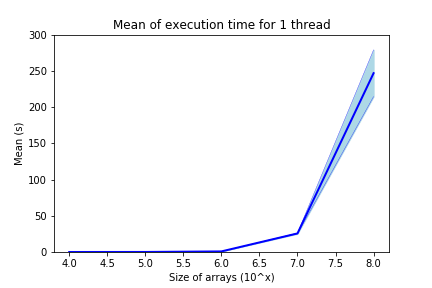
\includegraphics[width = 0.45\linewidth]{Mean of execution time for 1 thread.png}
        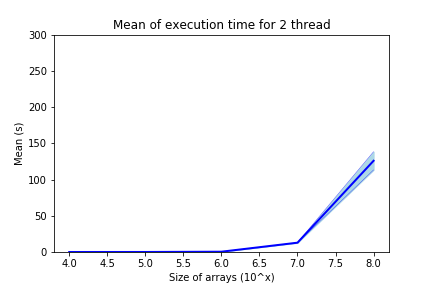
\includegraphics[width = 0.45\linewidth]{Mean of execution time for 2 thread.png}

    \end{figure}
    \begin{figure}[ht]
         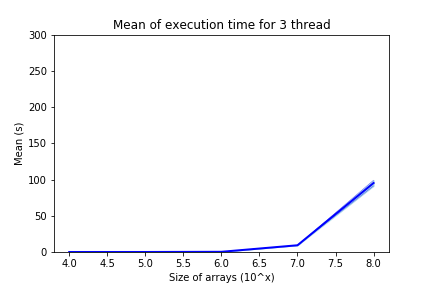
\includegraphics[width = 0.45\linewidth]{Mean of execution time for 3 thread.png}
        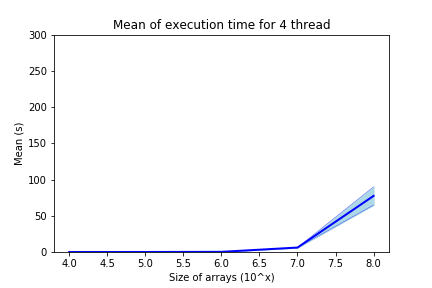
\includegraphics[width = 0.45\linewidth]{Mean of execution time for 4 thread.png}
        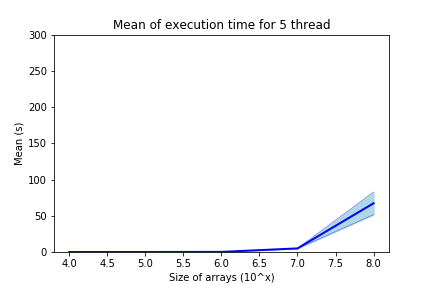
\includegraphics[width = 0.45\linewidth]{Mean of execution time for 5 thread.png}
        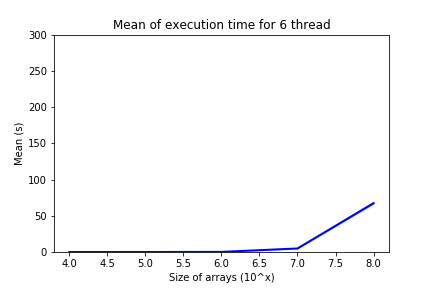
\includegraphics[width = 0.45\linewidth]{Mean of execution time for 6 thread.png}
        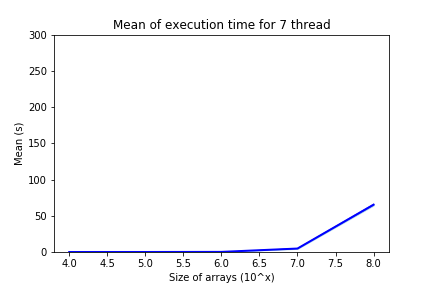
\includegraphics[width = 0.45\linewidth]{Mean of execution time for 7 thread.png}
        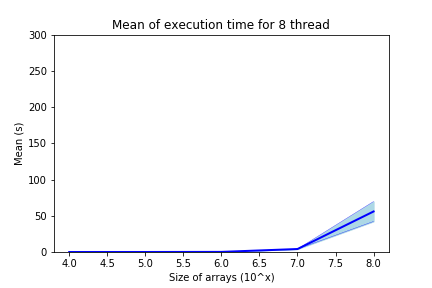
\includegraphics[width = 0.45\linewidth]{Mean of execution time for 8 thread.png}
        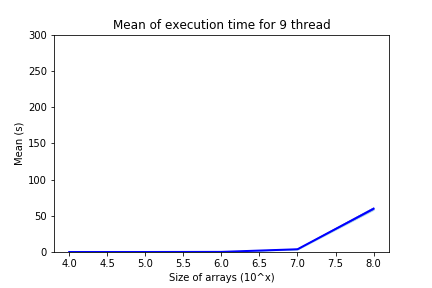
\includegraphics[width = 0.5\linewidth]{Mean of execution time for 9 thread.png}
        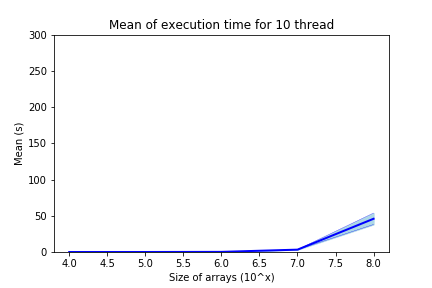
\includegraphics[width = 0.5\linewidth]{Mean of execution time for 10 thread.png}
    \end{figure}

    
\newpage

    \begin{figure}
    
        \centering
        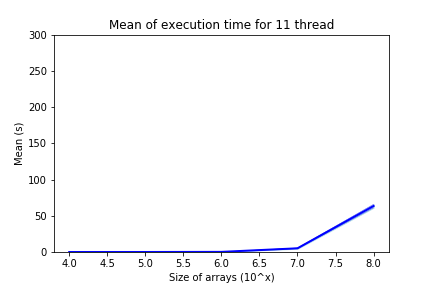
\includegraphics[width = 0.45\linewidth]{Mean of execution time for 11 thread.png}
        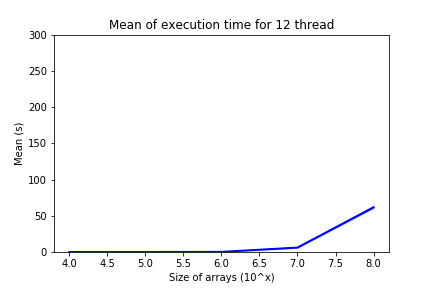
\includegraphics[width = 0.45\linewidth]{Mean of execution time for 12 thread.png}
        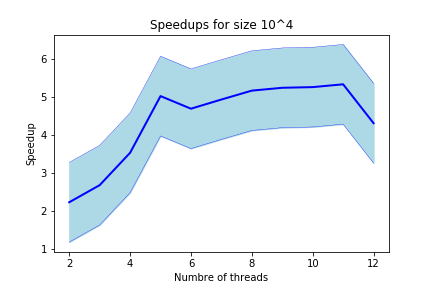
\includegraphics[width = 0.45\linewidth]{Speedups for size 10^4.png}
        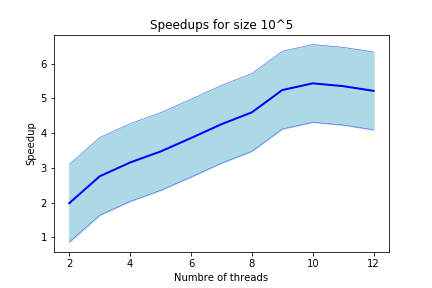
\includegraphics[width = 0.45\linewidth]{Speedups for size 10^5.png}
        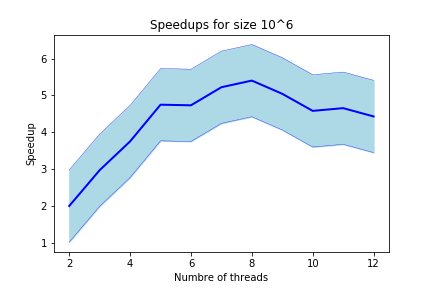
\includegraphics[width = 0.45\linewidth]{Speedups for size 10^6.png}
        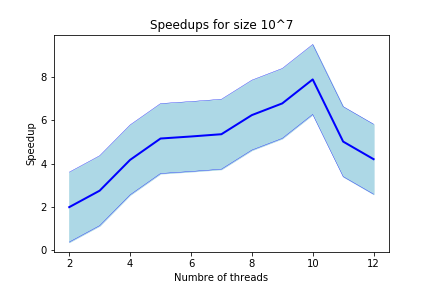
\includegraphics[width = 0.45\linewidth]{Speedups for size 10^7.png}
        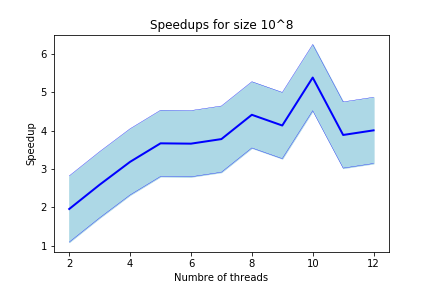
\includegraphics[width = 0.55\linewidth]{Speedups for size 10^8.png}
    \end{figure}



\end{document}